% !TEX root = ../Dokumentation.tex
\subsection{Lenkung}
\textbf{Funktionsbeschrieb}\\[0.2cm]
Die Lenkung ist eine Achsschenkellenkung. Sie wird heute in fast allen PKWs, LKWs, Omnibussen und sonstigen Nutzfahrzeugen eingesetzt. Bei dieser Art der Lenkung befinden sich die Räder auf einzeln lenkbaren Achsschenkeln, die jeweils mit einem Spurstangenhebel versehen sind. Die Spurstangenhebel sind ungefähr senkrecht zur Vorderachse bzw. ungefähr parallel zur Längsachse des Fahrzeugs ausgerichtet und durch eine Spurstange miteinander verbunden. Deshalb ist es möglich beide Räder gleichzeitig zu lenken.\\[0.2cm]
\textbf{Komponentenbeschrieb}\\[0.2cm]
Mit einem Servomotor wird über eine Kegelradverbindung der Lenkschubhebel angetrieben. Dieser treibt wiederum die Spurstange an, welche die Bewegung über die Spurstangenhebel an die Räder weitergibt.
\begin{figure}[H]%Position festigen
\centering
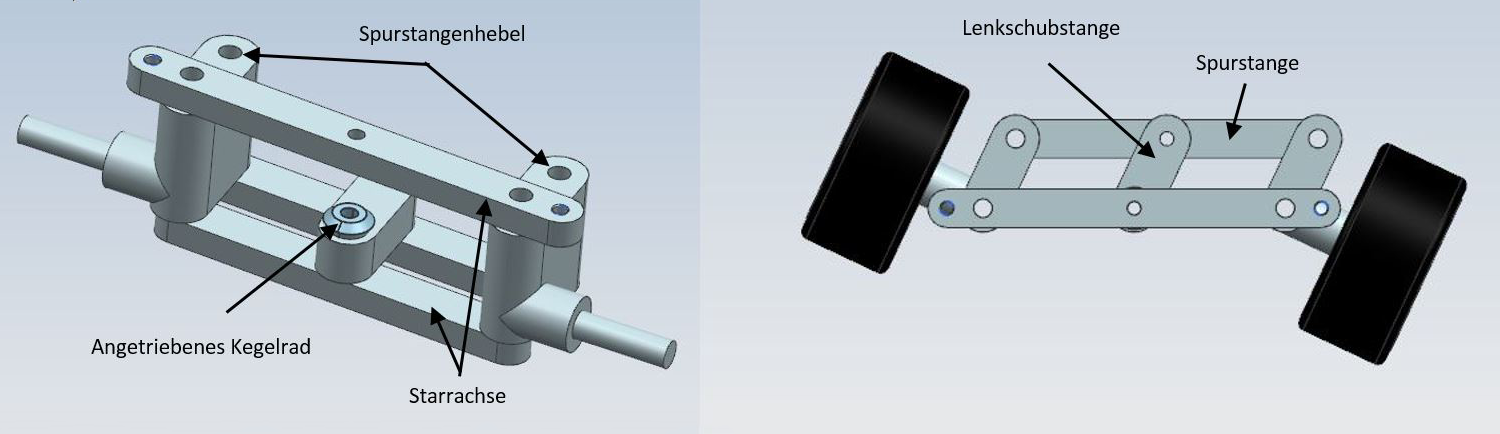
\includegraphics[width=1\textwidth]{03_Loesungskonzept/pictures/Achsschenkellenkung.png}
\caption{Konzept der Achsschenkellenkung}
\label{fig:activityRoute}
\end{figure}
\textbf{Begründung}\\[0.2cm]
Für die Bildverarbeitung ist das Lenken und das konstante Ausgleichen der Fahrbahn und Fahrtgeschwindigkeit mit zwei Motoren, welche jeweils ein Rad antreiben ein Nachteil. Darum ist das Lösungskonzept mit einer Achsschenkellenkung ausgestattet. Von der konstruktiven Seite ist die Achsschenkellenkung im Vergleich zwar aufwändiger, aber für die Aufgabenstellung besser geeignet. Da es das Ziel ist, einen möglichst konstanten Abstand zum Trottoir der Fahrbahn zu halten, ist die Regelung einer Achsschenkellenkung einfacher. Weitere Gründe, welche für die Achsschenkellenkung sprechen, wurden schon im Kapitel \glqq{Chassis}\grqq{} erläutert.
Die Begründung für die Wahl des Servomotors ist, dass die Lenkung keine 360°-Bewegungen durchführen muss. Zudem ist die Drehzahl des Servos leicht zu steuern, ohne dass zusätzlich eine Regelung eingebaut werden muss. \\[0.2cm]
\textbf{Berechnungen}\\[0.2cm]
Berechnung Drehmoment Servo Lenkung
\begin{itemize}
\item Gewichtskraft auf jedes Rad $Fg = \frac{m\cdot g}{4}$
\item Abstand $l = 30mm$
\item $M = 2\cdot Fg\cdot l = 0.37Nm$
\item Sicherheitsfaktor = 1.5 (da Beschleunigung- und Bremskräfte vernachlässigt werden)
\item $M = 0.37\cdot 1.5 = 0.555Nm = 55.5Ncm$
\end{itemize}